% Type-Token Ratio Comparison
% Add to main.tex after \begin{document}

\begin{figure}[t]
\centering
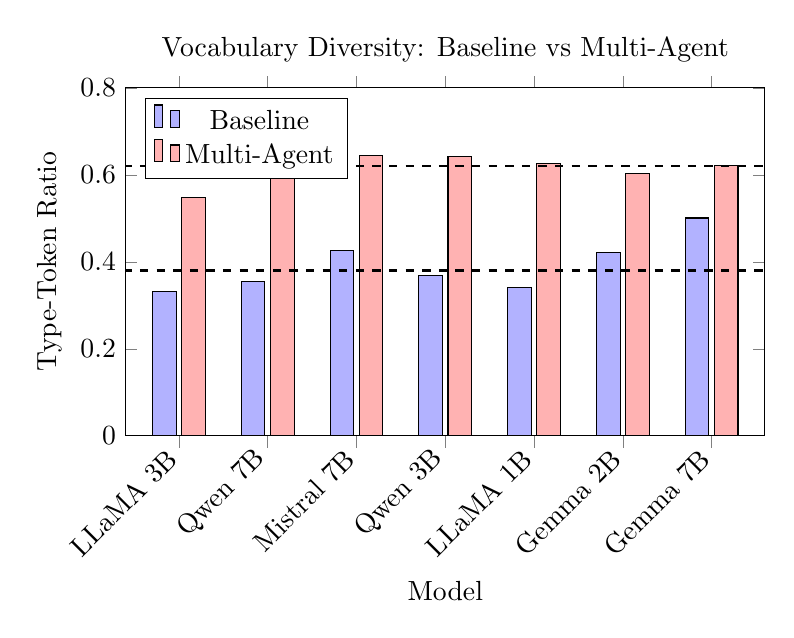
\begin{tikzpicture}
\begin{axis}[
    width=0.8\textwidth,
    height=6cm,
    ybar,
    bar width=0.3cm,
    xlabel={Model},
    ylabel={Type-Token Ratio},
    ymin=0, ymax=0.8,
    xtick={1,2,3,4,5,6,7},
    xticklabels={LLaMA 3B, Qwen 7B, Mistral 7B, Qwen 3B, LLaMA 1B, Gemma 2B, Gemma 7B},
    x tick label style={rotate=45, anchor=east},
    legend pos=north west,
    title={Vocabulary Diversity: Baseline vs Multi-Agent}
]

% Baseline TTR
\addplot[fill=blue!30] coordinates {
    (1, 0.3322)
    (2, 0.3549)
    (3, 0.4259)
    (4, 0.3693)
    (5, 0.3404)
    (6, 0.4221)
    (7, 0.5008)
};

% Multi-agent TTR
\addplot[fill=red!30] coordinates {
    (1, 0.5476)
    (2, 0.6453)
    (3, 0.6444)
    (4, 0.6427)
    (5, 0.6267)
    (6, 0.6025)
    (7, 0.6223)
};

\legend{Baseline, Multi-Agent}

% Average line
\draw[dashed, thick, black] (axis cs:0,0.38) -- (axis cs:8,0.38);
\node[right] at (axis cs:7.5,0.38) {Baseline Avg: 0.38};

\draw[dashed, thick, black] (axis cs:0,0.62) -- (axis cs:8,0.62);
\node[right] at (axis cs:7.5,0.62) {Agent Avg: 0.62};

\end{axis}
\end{tikzpicture}
\caption{Type-Token Ratio (TTR) comparison measuring vocabulary diversity. Multi-agent outputs show 63\% higher TTR (0.62 vs 0.38), indicating more diverse vocabulary usage despite being shorter.}
\label{fig:ttr}
\end{figure}
